\begin{figure}
\begin{center}
    \centering
    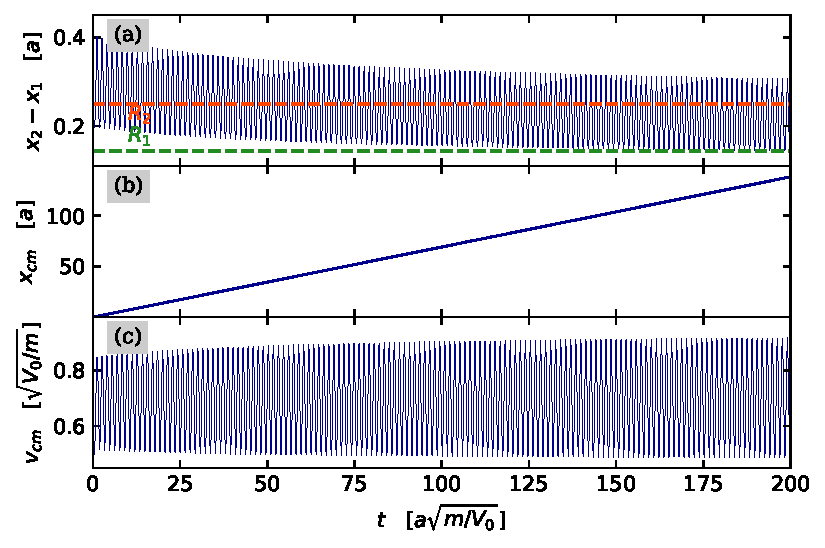
\includegraphics[width=1\linewidth]{Images/11_a_R_Xcm.pdf}
    \caption{Oscillations covering both the $R_1$ maximum and the $R_2$ minimum of the potential $V_\text{int}$, occurring with $R_1 = \frac{\sqrt{3}}{12} a$, $R_2 = 0.25 a$, $F = 7.5 \f$, $\gamma = 10 \g$, $ U = 1 \p$ and therefore $\delta = 3.6169 \times 10^{-5} V_0$ and initial condition $R_0=R_2$. \textbf{(a)} relative coordinate $r$; \textbf{(b)} center of mass $x_\text{cm}$; \textbf{(c)} velocity of the center of mass $v_\text{cm}$. }
    \label{Fig:11_a_R_Xcm}
\end{center}
\end{figure}

\begin{figure}
\begin{center}
    \centering
    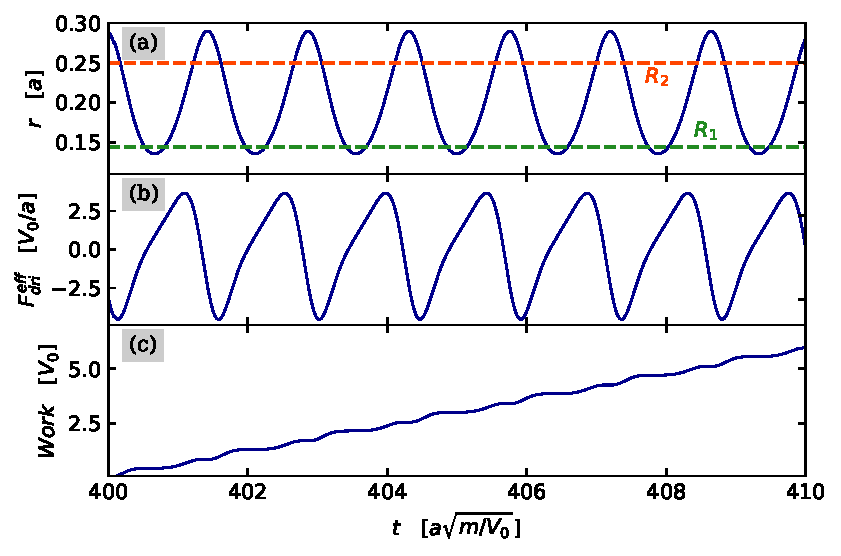
\includegraphics[width=1\linewidth]{Images/11_a_R_Forzante_2.pdf}
    \caption{\textbf{(a)} A blowup of a portion of the motion for the relative coordinate $r = |x_2 - x_1|$, as already reported in Fig.~\ref{Fig:11_a_R_Xcm}. \textbf{(b)} Effective driving force acting on this relative coordinate $F_{\text{dri}}^{\text{eff}}$, as given by Eq.~\eqref{eq:driving}. It can be seen that the force and the motion have the same frequency, and that the phase of the displacement is delayed by approximately 90° relative to the driving force. \textbf{(c)} Work of $F_{\text{dri}}^{\text{eff}}$. $W = \int_{t_0}^t F_{\text{dri}}^{\text{eff}}(t') \dot{r}(t') dt' $. We take $t_0 = 400 \tim$, safely after the initial non-periodic stage of the motion. }
    \label{Fig:11_a_R_Forzante}
\end{center}
\end{figure}


\begin{figure}
\begin{center}
    \centering
    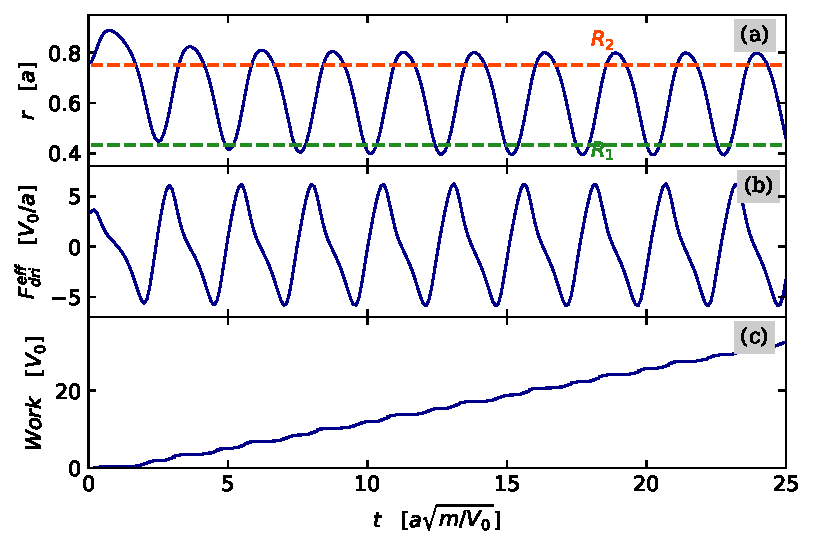
\includegraphics[width=1\linewidth]{Images/11_b_R_Forzante_2.pdf}
    \caption{Same as Fig.~\ref{Fig:11_a_R_Forzante} but with $R_1 = \frac{\sqrt{3}}{4} a$, $R_2 = \frac{3}{4} a$, $F = 5 \f$, $\delta = 2.6367 \times 10^{-2} V_0$, $R_0=R_2$. In panel \textbf{(c)} the work is integrated from $t_0 = 0 $.}
    \label{Fig:11_b_R_Forzante}
\end{center}
\end{figure}



Our first main objective is to identify an explanation for oscillations of the kind reported in Fig.~\ref{Fig:11_a_R_Xcm} and~\ref{Fig:11_b_R_Forzante} (a), also identified in Ref.~\cite{Cavallini}. These oscillations of the relative coordinate $r := |x_2 -x_1|$ are surprising because they seem not to be centered around a minimum of the molecular potential, but they span from a minimum to a local maximum, and even beyond it.

One can argue that the molecule has simply enough momentum to climb the potential barrier toward the maximum. However, this is not a valid argument for at least two reasons. The first one is that these oscillations are obtained in an overdamped regime, with $\gamma = 10 \g$.\footnote{A discussion about the values of $\gamma$ for which we can talk about an overdamped regime can be found in~\cite{Cavallini}, \S~4.1.} This large damping factor implies strong viscous friction, that makes all inertial movements rapidly disappear. This statement is confirmed by the second argument, i.e.\ that, as illustrated in Figs.~\ref{Fig:11_a_R_Forzante}a and~\ref{Fig:11_b_R_Forzante}a, the oscillation can extend even a little beyond the maximum at $R_1$. If inertia prevailed, then one would expect the molecule, once the barrier is climbed, to collapse to zero following the attractive force associated with $V_\text{int}$.

It must be now clear that a simple description based on a weakly driven oscillation around the minimum of $V_\text{int}$ is completely inadequate, and that is the motion along the periodic potential $V_\text{ext}$ that makes this peculiar behavior possible. A simple observation is that when $r$ has passed the maximum at $R_1$ and inverts his motion,
%mettere immagine chiara 
the two particles are found in different "valleys" of $V_\text{ext}$, i.e.\ the first is before one of the peaks, and the second is after. So the $x_1$ particle is pulled back to the left toward the previous minimum, and the $x_2$ particle is pushed forward. That favors an increase of their mutual distance $r$, that can effectively contrast the force generated by $V_\text{int}$. %magari formulare meglio: n esimo picco in na


But why do these oscillations occur only for some particular selections of the dynamical parameters? It is natural to require a reasonably small value of $\delta$ because if the forces generated by $V_\text{int}$ were too strong, it would be very difficult to climb the potential barrier and then not to collapse in the origin. Also, we already mentioned that a large damping factor helps quenching inertial effects. It is not trivial however to understand the role of $R_1$, $R_2$ and the external force $F$. We start by writing the Newton equation for the relative coordinate $r$:

%\begin{equation}
   % \mu\ddot{r} =  \overbrace{-\frac{V_0\pi}{a}\cos \left(\frac{2\pi x_\text{cm}}{a}\right)\sin\left(\frac{\pi r}{a}\right)}^{F_{\text{dri}}^{\text{eff}}} - V'_\text{int}(r) -2\gamma \mu \dot{r}
    %\label{eq:rdot}
%\end{equation}

\begin{equation}
    \mu\ddot{r} =  -\frac{V_0\pi}{a}\cos \left(\frac{2\pi x_\text{cm}}{a}\right)\sin\left(\frac{\pi r}{a}\right)- V'_\text{int}(r) -2\gamma \mu \dot{r},
    \label{eq:rdot}
\end{equation}
where $\mu = \frac{m_1m_2}{m_1+m_2}$ is the reduced mass of the molecule, that in our case of identical particles is equal to $m/2$. 
We can immediately make the following observations:
\begin{itemize}

    \item The motion of $r$ is coupled to that of the variable $x_\text{cm}$
    
    \item $F$ is not explicitly present in Eq.~\eqref{eq:rdot}, but it affects $r$ trough $x_\text{cm}$
    
    \item The $V'_\text{int}$ term is conservative, while the other force term
    \begin{equation}
         F_{\text{dri}}^{\text{eff}} :=-\frac{2V_0\pi}{a}\cos \left(\frac{2\pi x_\text{cm}}{a}\right)\sin\left(\frac{\pi r}{a}\right)
         \label{eq:driving}
    \end{equation}
    is responsible for pumping energy into the system. This energy is eventually dissipated by the final $\gamma$ term.
    
\end{itemize}


\begin{figure}
\begin{center}
    \centering
    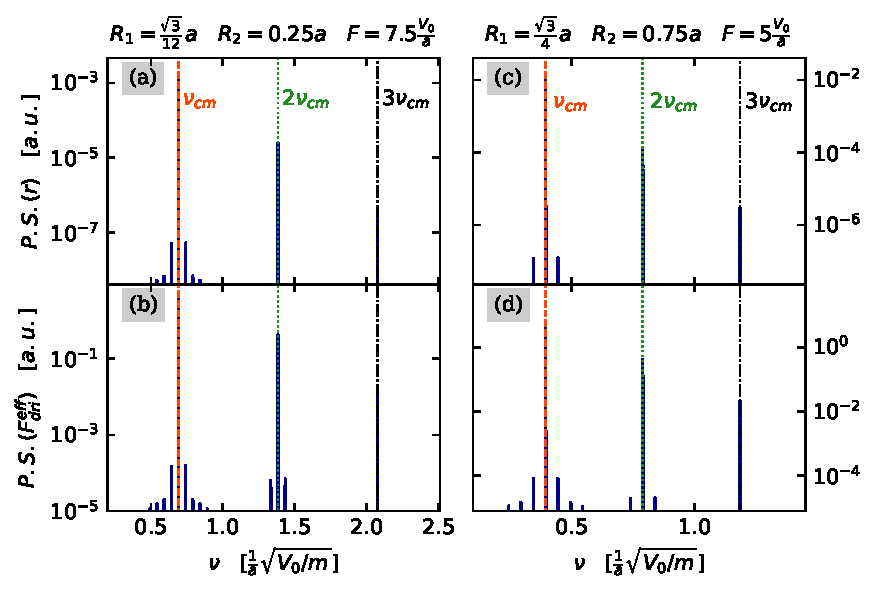
\includegraphics[width=1\linewidth]{Images/FFT.pdf}
    \caption{Power spectrum of the relative coordinate $r(t)$ and of the effective driving force $F_{\text{dri}}^{\text{eff}}(t)$ for the time sequences of: \textbf{(a)} Fig.~\ref{Fig:11_a_R_Forzante}a; \textbf{(b)} Fig.~\ref{Fig:11_a_R_Forzante}b; \textbf{(c)} Fig.~\ref{Fig:11_b_R_Forzante}a; \textbf{(d)} Fig.~\ref{Fig:11_b_R_Forzante}b. In all four spectra the peak corresponding to $\nu_\text{cm} = \Bar{v}_\text{cm}/a $ is dominant, followed by other weaker peaks at $2\nu_\text{cm}$ and $3\nu_\text{cm}$ representing the second and the third harmonic. Panels \textbf{(a,b)}:  $\nu_\text{cm} = 0.6927 \frac{1}{a}\sqrt{\frac{V_0}{m}}$; panels \textbf{(c,d)}:  $\nu_\text{cm} = 0.3950 \frac{1}{a}\sqrt{\frac{V_0}{m}}$.}
    \label{Fig:FFT}
\end{center}
\end{figure}

\begin{comment}
\begin{figure}
\begin{center}
    \centering
    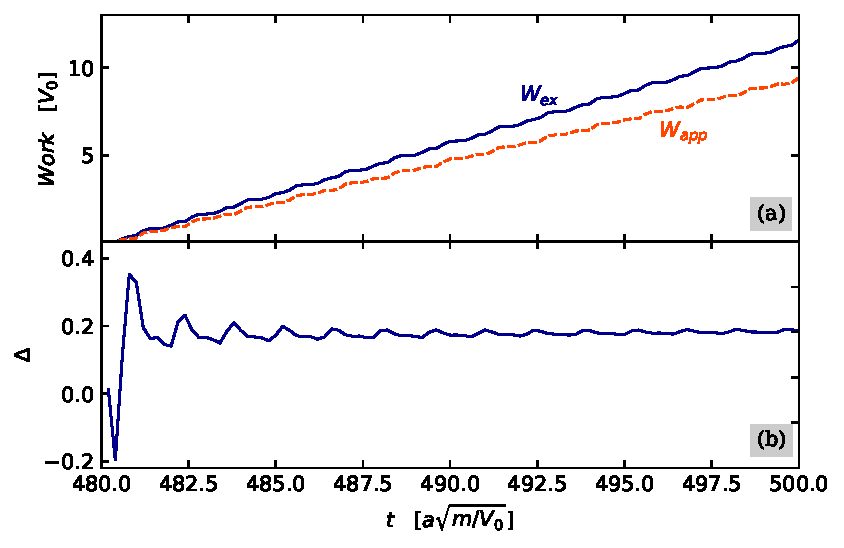
\includegraphics[width=1\linewidth]{Images/11_a_Work_b.pdf}
    \caption{Work of $F_{\text{dri}}^{\text{eff}}$ for the dynamics of Figs.~\ref{Fig:11_a_R_Xcm} and~\ref{Fig:11_a_R_Forzante}. $W = \int_{t_0}^t F_{\text{dri}}^{\text{eff}}(t') \dot{r}(t') dt' $. We take $t_0 = 480 \tim$, safely after the initial non periodic stage of the motion. \textbf{(a)} the solid line is the exact work $W_{ex}$, the dashed one is the approximate work $W_{app}$ obtained using the approximation of Eq.~\eqref{eq:coswt}; \textbf{(b)} relative error $\Delta = \frac{W_{ex}-W_{app}}{W_{ex}}$} 
    \label{Fig:11_a_Work}
\end{center}
\end{figure}

\begin{figure}
\begin{center}
    \centering
    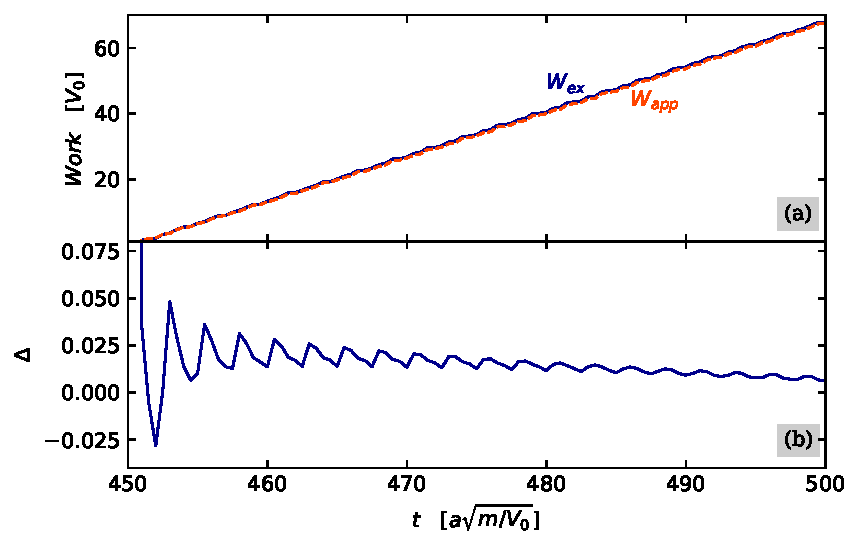
\includegraphics[width=1\linewidth]{Images/11_b_Work_b.pdf}
    \caption{Same as Fig.~\ref{Fig:11_a_Work} but for the oscillation of Fig.~\ref{Fig:11_b_R_Forzante} }
    \label{Fig:11_b_Work}
\end{center}
\end{figure}
\end{comment}

\subsection{The effective driving force}
We now focus on this effective driving force $F_{\text{dri}}^{\text{eff}}$, the force that drives these peculiar oscillations. Figures~\ref{Fig:11_a_R_Forzante} and~\ref{Fig:11_b_R_Forzante} show that, after the initial transient stage, the motion of $r$ oscillates at the same frequency of $F_{\text{dri}}^{\text{eff}}$, thus justifying the use of the term driving force. $F_{\text{dri}}^{\text{eff}}$ is the product of two oscillating terms, one dependent on $r$ itself and the other one on $x_\text{cm}$. Their combination can give rise to a complex time dependence of the effective force. Figures~\ref{Fig:11_a_R_Forzante}b and~\ref{Fig:11_b_R_Forzante}b show that $F_{\text{dri}}^{\text{eff}}$, after the initial transient stage, is a periodic function. 

We can first of all observe that (i) in a sliding (unpinned) state, $\cos \left(\frac{2\pi x_\text{cm}}{a}\right)$ spans all the values from -1 to +1; (ii) in the asymptotic oscillatory regime developed after the initial transient, if the oscillation is confined in a suitable limited region, $\sin\left(\frac{\pi r}{a}\right)$ ranges between $\sin\left(\pi\frac{ r_\text{min}}{a}\right)$ and $\sin\left(\pi\frac{ r_\text{max}}{a}\right)$, where $r_\text{min} \sim R_1$ and $r_\text{max} \sim R_2$ account for the oscillation range. For example, with the condition of Fig.~\ref{Fig:11_a_R_Forzante},
$ 0.39 < \sin\left(\frac{\pi r}{a}\right) < 0.81$; for the condition of Fig.~\ref{Fig:11_b_R_Forzante}, $ 0.59 < \sin\left(\frac{\pi r}{a}\right) < 0.95$. In these examples, this term never changes sign during the oscillation, and just modulates the main oscillatory term $\cos \left(\frac{2\pi x_\text{cm}}{a}\right)$. We can observe from Fig.~\ref{Fig:11_a_R_Xcm} (b,c) that the motion of $x_\text{cm}$ resembles a rectilinear uniform advancement, with small oscillations. Indeed $v_\text{cm}$ is not quite constant, but, after the initial transient, it oscillates around a mean constant value. If we neglect this small oscillation, we obtain the following approximation for this oscillatory term in $F_{\text{dri}}^{\text{eff}}$:
\begin{equation}
    \cos \left(\frac{2\pi x_\text{cm}}{a}\right) \approx \cos \left(\frac{2\pi \Bar{v}_\text{cm}}{a}t\right) = \cos\left(2\pi \nu_\text{cm}t\right) = \cos \left(\omega_\text{cm} t\right).
    \label{eq:coswt}
\end{equation}
In this equation, $\Bar{v}_\text{cm}$ is the mean velocity of the center of mass. Correspondingly, $\nu_\text{cm} = \Bar{v}_\text{cm}/a$ is the washboard frequency for the molecule advancing over the periodic corrugation. We then expect the frequency of $F_{\text{dri}}^{\text{eff}}$ and of the oscillation of $r$ to be exactly $\nu_\text{cm}$. This observation can be confirmed by a Fourier analysis. Figure~\ref{Fig:FFT} report the power spectrum, obtained as the squared modulus of its Fourier transform. The power spectrum of a quantity $y(t)$ is computed by
\begin{equation}
    P.S.(y)[\nu] = \left|\frac{1}{N}\sum_{n=1}^N e^{-2\pi i \frac{\nu n \Delta t}{N}}y[n \Delta t]\right|^2.
    \label{eq:ps}
\end{equation}
%This results in a peak in the origin for Fig.~\ref{Fig:FFT} (a) and (b), that is not reported.

%Another confirmation of the goodness of our approximation comes by looking at the energy pumped in the system by $F_{\text{dri}}^{\text{eff}}$, that we expect to be positive to balance the dissipation given by $\gamma \dot{r}$. In Figs.~\ref{Fig:11_a_Work} and~\ref{Fig:11_b_Work} are reported for both oscillations studied the work of the exact and approximate expression of $F_{\text{dri}}^{\text{eff}}$, and their normalized difference. The results are good in both cases, but especially for Fig.~\ref{Fig:11_b_Work}. For longer periods of integration the results can worsen significantly, because the approximate expression of $F_{\text{dri}}^{\text{eff}}$ can assume a different phase relative to $\dot{r}$, resulting even in an inversion of the trend of $W_{app}$, that starts decreasing.

\begin{figure}
\begin{center}
    \centering
    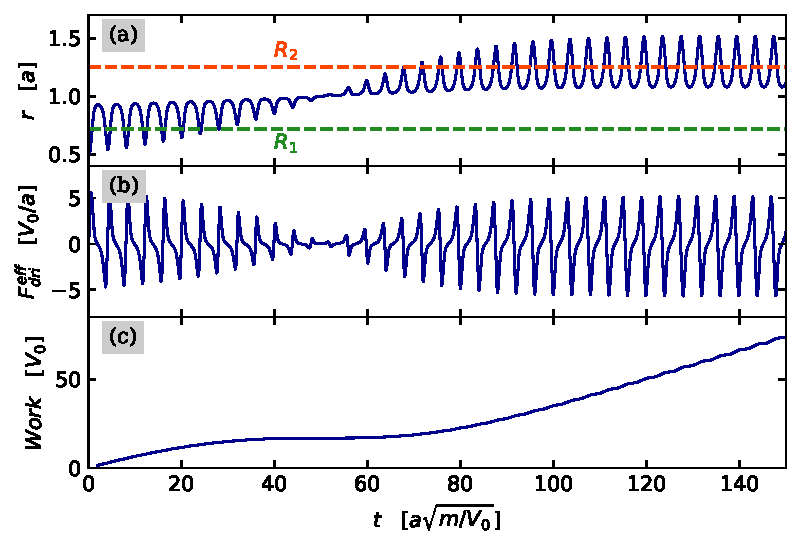
\includegraphics[width=1\linewidth]{Images/12_a.pdf}
    \caption{Example of dynamics in a condition where $R_1 < a < R_2$, implying a sign change of the $\sin \left(\frac{\pi r}{a}\right)$ term. $R_1 = 5\frac{\sqrt{3}}{12} a$, $R_2 = 1.25 a$,  $F = 4 \f$, $\gamma = 10 \g$, $ U = 0.01 \p$ (so that $\delta = 5.6514 \times 10^{-3} V_0$), initial condition $R_0= 0.5 a$. \textbf{(a)} relative coordinate $r$; \textbf{(b)} effective driving force $F_{\text{dri}}^{\text{eff}}$; \textbf{(c)} exact work done by $F_\text{dri}^{\text{eff}}$ on the internal degree of freedom. }
    \label{Fig:12_a}
\end{center}
\end{figure}

\begin{figure}
\begin{center}
    \centering
    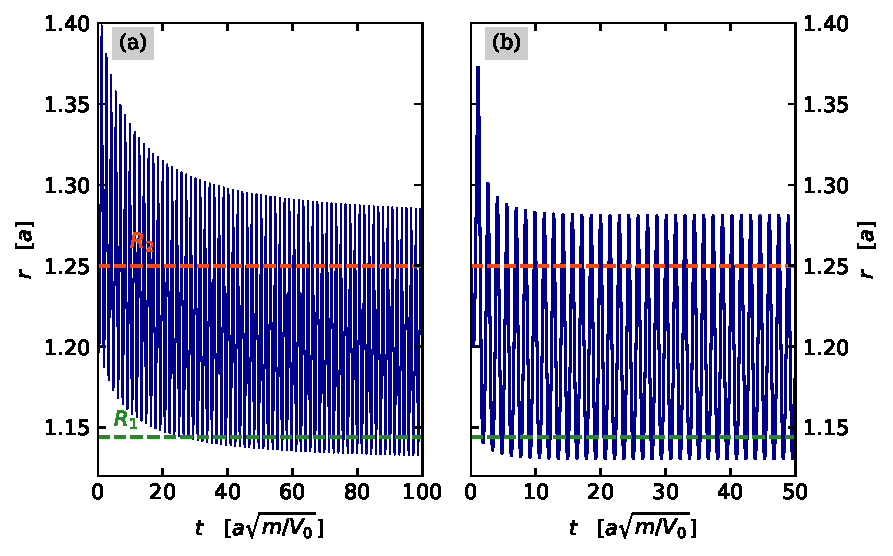
\includegraphics[width=1\linewidth]{Images/1.14434.pdf}
    \caption{Oscillations covering the maximum at $R_1 = 1.14434 a$ and the minimum at $R_2 = 1.25 a$. The simulation parameters are $\gamma = 10 \g$, $F = 7.5 \f$, and the initial condition is $R_0=R_2$. The other parameters are: \textbf{(a)} $U = 0.1 \p$ (so that $\delta = 8.0958 \times 10^{-4} V_0$); \textbf{(b)} $U = 1 \p$ ($\delta = 8.0958 \times 10^{-3} V_0$).}
    \label{Fig:1.14434}
\end{center}
\end{figure}

\begin{figure}
\begin{center}
    \centering
    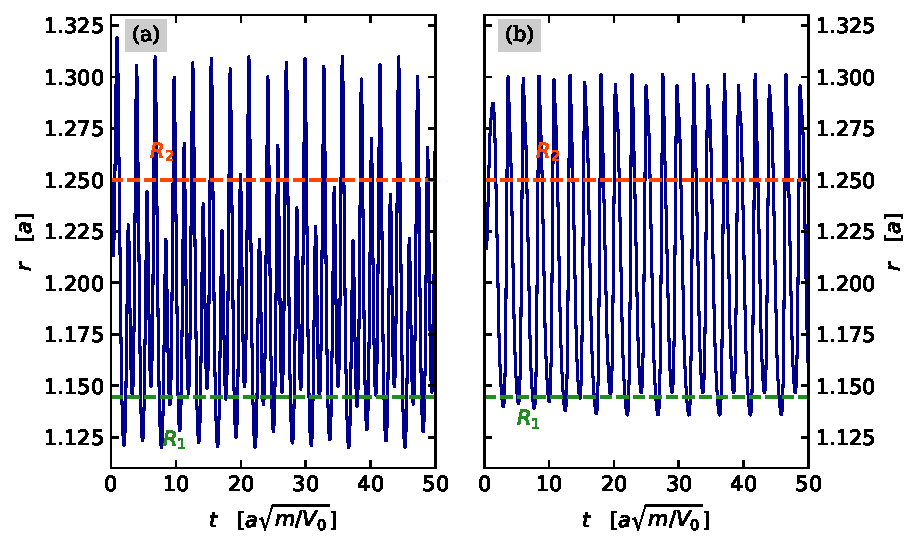
\includegraphics[width=1\linewidth]{Images/1.14434_b.pdf}
    \caption{Same as Fig.~\ref{Fig:1.14434}, but with \textbf{(a)} $F = 7.5 \f$, $U = 5 \p$ ($\delta =  4.0479\times 10^{-2} V_0$); \textbf{(b)} $F = 5.05 \f$, $U = 10 \p$ ($\delta =  8.0958\times 10^{-2} V_0$);}
    \label{Fig:1.14434_b}
\end{center}
\end{figure}

\subsection{Sign changes in $\sin(\pi r /a)$}
We are now convinced that $F_{\text{dri}}^{\text{eff}}$ plays a central role in driving the desired oscillations, and that the frequency of the latter is the same as the mean center of mass washboard frequency. From Figs.~\ref{Fig:11_a_R_Forzante}c and~\ref{Fig:11_b_R_Forzante}c, we can see that the work of $F_{\text{dri}}^{\text{eff}}$ is  monotonically increasing to sustain the oscillation. We then hypothesize that it helps that the term $\sin\left(\frac{\pi r}{a}\right)$ does not vanish nor change its sign during the oscillation. This is equivalent to ask that between $R_1$ and $R_2$ there are no points of the type $r = na$ with $n = 0, \pm1, \pm2 ...$

We investigate what happens when this condition is violated. Such a situation is reported in Fig.~\ref{Fig:12_a}. We see that when $r=a$, the effective driving force vanishes, and stops pumping energy into the molecule, leading to a small-amplitude oscillation in a neighborhood of $R_2$, where $F_{\text{dri}}^{\text{eff}}$ oscillates with sufficient amplitude. Thus a stable oscillation between $R_1$ and $R_2$ is not possible, and the oscillation around $R_2$ cannot extend beyond $r=a$, the point where $F_{\text{dri}}^{\text{eff}}$ vanishes.

As a limiting case, if we move this force-vanishing point to $R_2 = na$, no oscillations are sustained, and the molecule collapses to $R_2$, in a similar way as it collapses to the origin, giving a suitably small initial condition $R_0$. 

\subsection{Negative values of $\sin(\pi r /a)$}
We want to check what happens when the term $\sin\left(\frac{\pi r}{a}\right)$ assumes negative values. We then do a translation by $a$ of the spatial parameters $R_1$ and $R_2$ of the case of Figs.~\ref{Fig:11_a_R_Xcm} and~\ref{Fig:11_a_R_Forzante}. Doing so, the term $\sin\left(\frac{\pi r}{a}\right)$ is always negative between $R_1$ and $R_2$, with no vanishing points. For suitable values of $U$ and $F$, we observe the same kind of broad amplitude oscillation exceeding the maximum at $R_1$, as shown in Fig.~\ref{Fig:1.14434}. This proves that the sign of the term $\sin\left(\frac{\pi r}{a}\right)$ does not matter, as long as it remains the same during the entire oscillation. 

\subsection{Higher values of the potential barrier $\delta$}
We now want to check how the strength of $V_\text{int}$ affects the oscillations. We then proceed by increasing $U$, and therefore $\delta$, obtaining the desired oscillations until $U=10 \p$ and $\delta =  8.0958\times 10^{-2} V_0$. We can see however from Fig.~\ref{Fig:1.14434_b} that with this value of the barrier the oscillations follow more intricate patterns. Actually, after the initial transient, a Fourier analysis shows that their frequency is $\nu_\text{cm}/2$, corresponding to a period doubling, relative to the washboard period. These oscillations become more regular increasing the value of $F$, but their amplitude decreases with the driving force, so that eventually they cannot reach $R_1$. With a higher value of $U$ such as $15 \p$, corresponding to $\delta = 0.12144 V_0$ , $R_1$ is never reached. 
We noted that when $\delta$ increases, the minimum value of $F$ for which a stable oscillation can be established decreases. \\

Studying the oscillations covering both $R_1$ and $R_2$ presented in this section, we noted that after having reached a value of $F$ large enough to sustain these oscillations, if we further increase the external force, the amplitude of the oscillations decreases. Decreasing $F$, the oscillation switches with continuity from spanning over $R_1$ to remaining confined outside the barrier at $R_1$. We can therefore interpret these oscillations between the maximum and the minimum of $V_\text{int}$ as simple oscillations around the minimum at $R_2$, but with enough amplitude to climb the potential barrier at R1, as long as it is sufficiently weak.


%In general, for all the oscillations presented in this section, Here we have said that for increasing $F$, the amplitude of the oscillations becomes smaller and smaller. We will study in detail the dependence of the amplitude of an oscillation around $R_2$ on the external force in the next section. 
 
 %For the choice of dynamical parameters of Fig.~\ref{Fig:1.14434}, for forces smaller than $7.5 \f$, the system collapses in the origin after some oscillations, and for bigger forces, the oscillation around $R_2$ becomes smaller and smaller. The fact that   leads us to see these oscillations between the maximum and the minimum of $V_\text{int}$ as simple oscillations around the minimum at $R_2$, but with enough amplitude to climb the potential wall $\delta$ in case it is quite small.